\documentclass[aspectratio=169]{beamer}

% beamer config
\usetheme{Pittsburgh}
\AtBeginSection{\frame{\sectionpage}}

% package imports
\usepackage{graphicx}
\graphicspath{{./figs/}}

% Macros
\newcommand{\todo}[1]{\textcolor{red}{\textbf{[#1]}}}

\title[PhotoHunter]{PhotoHunter: A Citizen-Scientist Game with User-in-the-loop 
  Data Confirmation for Collecting Computer Vision Datasets of 
  Geo-tagged Imagery through Crowd-Sourcing Data Collection; 
  Abstracting Research using an Interactive, Game-based Mobile 
  Application for Large Dataset Creation}

\author[]{Connor Greenwell \and Ryan Baltenberger 
  \and J.\ David Smith \and Aaron Bradshaw}

\institute{QuesoTech.com}

\begin{document}

\maketitle

\section{Computer Vision}

\begin{frame}
  As in other fields related to Artificial Intelligence or Machine
  Learning, having data to train or test on is integral to the success
  of Computer Vision projects. In Computer Vision, these datasets are 
  collections of images or videos, each with
  associated metadata. For example, in \cite{islam2014geofaces} they
  propose a collection of front-facing facial images each with an
  accompanying latitude-longitude pair. 

  What \cite{islam2014geofaces} and many others have in common
  is the difficulty they experienced when collecting these datasets.
  In
  this document, and the following sections we will propose a system
  for
  reducing these difficulties by proposing a system for crowd-sourcing
  images and videos, along with an 
\end{frame}

\section{Citizen-Science}

\begin{frame}
  Citizen-science is a form of crowdsourcing in which participants
  collect or analyze data. Typically, the tasks they perform are
  simple
  in nature. For example, they may be asked to take a photo, measure
  the 
  temperature, or translate text.

  This model is successful due to the ability of humans to perform
  such
  tasks extremely easily and in large numbers, often at little to no
  cost in time or effort. For a single research team to collect such
  large amounts of data on their own would be both costly and time
  consuming. Often, automating these tasks is impossible for
  computers,
  or is in fact the very aim of a projects principle investigators.
\end{frame}

\section{Why a game?}

\begin{frame}
  One of the drawbacks of citizen-science style is the sharp fall-off
  in
  user contributions as the initial interest wears off. One way to
  mitigate this decline in contribution is to ``game-ify'' the
  process.
  By abstracting out the actual data collection and telling users they
  are participating in a global scale scavenger hunt, we expect that
  users will stay engaged and, more importantly, keep contribuing data
  for scientists to study.

  Part of ``game-ify-ing'' PhotoHunter will involve assigning point
  values for both collecting and reviewing data. The users interaction
  with the website should be short, sweet, and rewarding. One of the
  ways to reward users is the use of a leaderboard.
\end{frame}

\section{Overview}

\begin{frame}
  \todo{Flowchart}
\end{frame}

\section{Backend}

\begin{frame}
  Research groups may be created on request. 

  Research groups will have an interface where they may request
  datasets. From this interface groups may define GPS bounding boxes,
  time frames, and other metadata they are interested in for a given
  dataset.
\end{frame}

\begin{frame}
  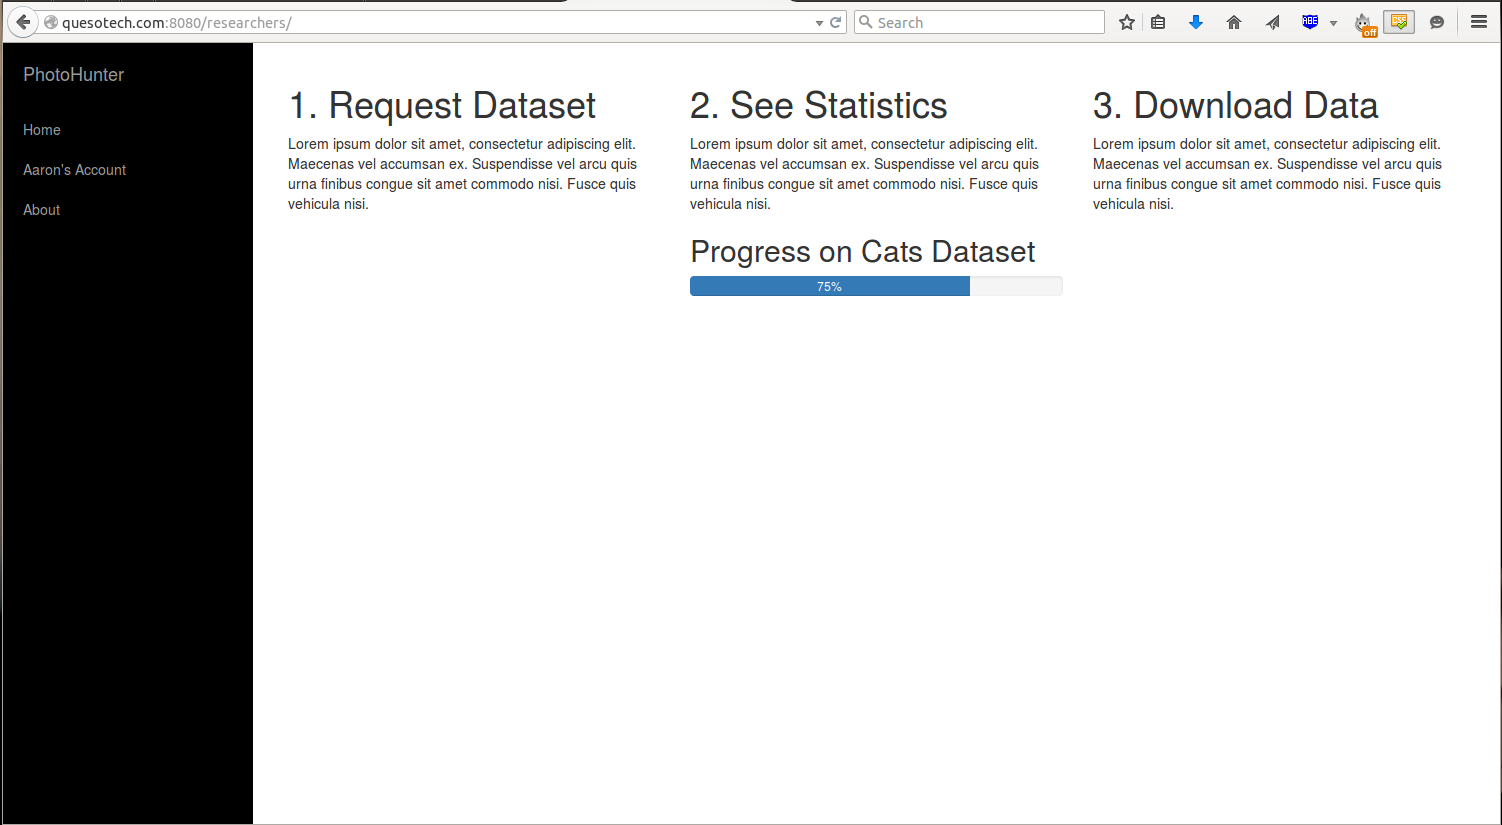
\includegraphics[width=\columnwidth]{researchers}
\end{frame}

\begin{frame}
  \todo{mockups}
\end{frame}

\begin{frame}
  \todo{ER diagrams}
\end{frame}

\section{PhotoHunter}

\begin{frame}
  From the mobile app, users will be presented with a list of
  datapoints
  to go collect in their area, and a time limit in which each must be
  completed. As each task is completed, they will gain points,
  prompting
  them to continue.

  Data collection will only occur within the mobile app so that we may
  take advantage of built in sensors (time, gps, heading, etc.).
\end{frame}

\begin{frame}
  \begin{columns}[c]
    \begin{column}{0.5\columnwidth}
      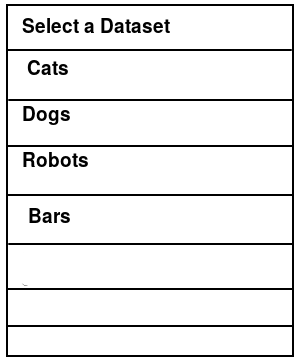
\includegraphics[width=\columnwidth]{ss_photohunter_dataset}
    \end{column}
    \begin{column}{0.5\columnwidth}
      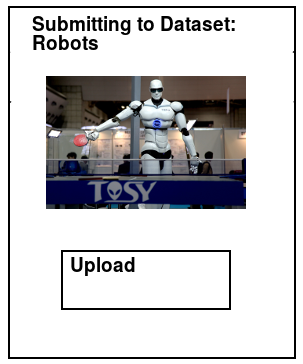
\includegraphics[width=\columnwidth]{ss_photohunter_upload}
    \end{column}
  \end{columns}
\end{frame}

\section{QuickPic}

\begin{frame}
  For numerous reasons, users may unknowingly (or knowingly) submit
  incorrect data. For example, a dataset that is seeking pictures of
  fire hydrants may accidentally receive images of dogs, or trees. In
  this case we will employ users to filter submissions. When an image
  is
  submitted, it will be posted for confirmation by other users. The
  interface for this will display the image in question, the
  requirements, and a simple ``thumbs-up'' and ``thumbs-down'' option.
  Each image will be presented for confirmation to numerous users
  until
  we can be reasonably certain that the datapoint should be trusted.
\end{frame}

\begin{frame}
  \begin{columns}[c]
    \begin{column}{0.5\columnwidth}
      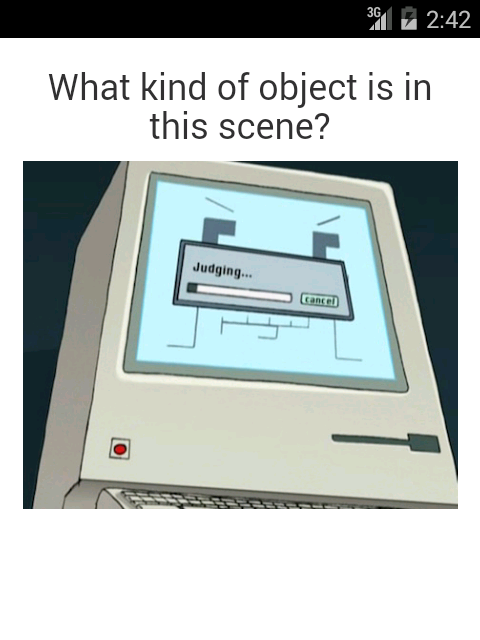
\includegraphics[width=\columnwidth]{ss_quickpic_image}
    \end{column}
    \begin{column}{0.5\columnwidth}
      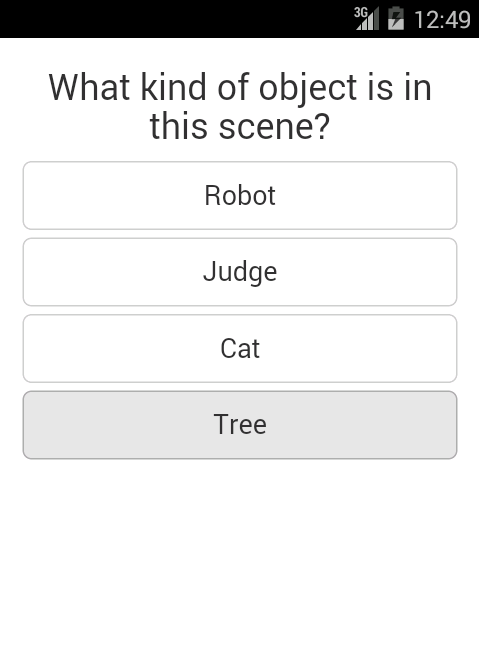
\includegraphics[width=\columnwidth]{ss_quickpic_options}
    \end{column}
  \end{columns}
\end{frame}

\frame{\centering Thanks!}

\end{document}
